\documentclass[tikz]{standalone}

\usepackage[latin1]{inputenc}
\usepackage{tikz}

% GNuPL
\begin{document}
\pagestyle{empty}


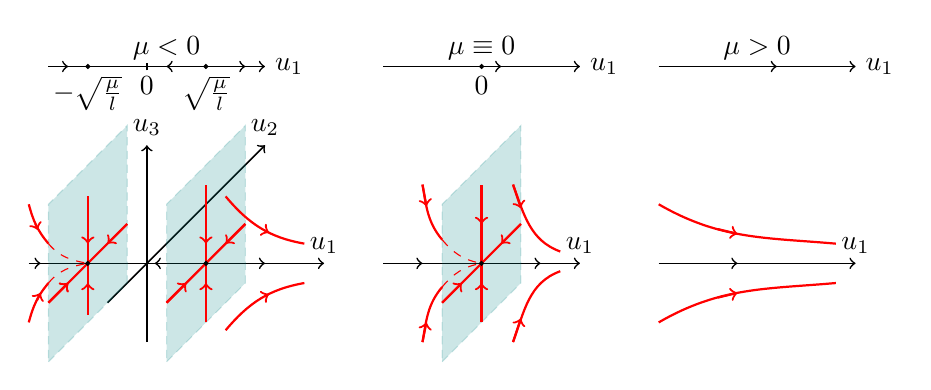
\begin{tikzpicture}[scale=0.5]
    %\mu<0
    \coordinate [label=-90:$\mu<0$] (8) at (3.5,9);

    \draw[semithick] [->] (0.5,8) -- (6,8) node[right] {$u_1$};
    \draw[semithick] [->] (0.5,8) -- (1,8);
    \draw[semithick] [->] (4.5,8) -- (3.5,8);
    \draw[semithick] [->] (4.5,8) -- (5.5,8);
    \draw [fill] (1.5,8) circle [radius=0.05];
    \draw [fill] (4.5,8) circle [radius=0.05];
    \draw[semithick] (3,7.9) -- (3,8.1);
    \coordinate [label=-90:$-\sqrt{\frac{\mu}{l}}$] (8) at (1.5,8);
    \coordinate [label=-90:$\sqrt{\frac{\mu}{l}}$] (8) at (4.5,8);
    \coordinate [label=-90:$0$] (8) at (3,8);


    \draw[semithick] [->] (0,3) -- (7.5,3) node[above] {$u_1$};
    \draw[semithick] [->] (0,3) -- (0.3,3);
    \draw[semithick] [->] (3.5,3) -- (3.2,3);
    \draw[semithick] [->] (5.8,3) -- (6,3);
	\draw[semithick] [->] (3,1) -- (3,6) node[above] {$u_3$};
	\draw[semithick] [->] (2,2) -- (6,6) node[above] {$u_2$};
	\draw[teal, densely dashed][fill = teal, opacity=0.2]  (0.5,0.5) -- (2.5,2.5) -- (2.5,6.5) -- (0.5,4.5) -- (0.5,0.5);
	\draw[teal,densely dashed][fill = teal, opacity=0.2]  (3.5,0.5) -- (5.5,2.5) -- (5.5,6.5) -- (3.5,4.5) -- (3.5,0.5);
	\draw [red, thick] (1.5,1.7) -- (1.5,3);
	\draw [red, thick] (0.5,2) -- (1.5,3);
	\draw [red, thick] (2.5,4) -- (1.5,3);
	\draw [red, thick] (1.5,4.7) -- (1.5,3);
	\draw [red, thick] [->] (0.5,2) -- (1,2.5);
	\draw [red, thick] [->] (2.5,4) -- (2,3.5);
	\draw [red, thick] [->] (1.5,2) -- (1.5,2.5);
	\draw [red, thick] [->] (0.5,2) -- (1,2.5);
	\draw [red, thick] [->] (1.5,4) -- (1.5,3.5);
    \draw [red,thick] (0,1.5) to [out=75,in=-130] (0.5,2.5);
    \draw [red, thick] [->] (0.2,2.05) -- (0.3,2.25);
    \draw [red,dashed] (0.5,2.5) to [out=50,in=-170] (1.5,3);  
    \draw [red,thick] (0,4.5) to [out=-75,in=130] (0.5,3.5);
    \draw [red, thick] [->] (0.17,4.) -- (0.23,3.85);
    \draw [red,dashed] (0.5,3.5) to [out=-50,in=170] (1.5,3);  	
	\draw [fill] (1.5,3) circle [radius=0.05]; 
	\draw [red, thick] (3.5,2) -- (4.5,3);
	\draw [red, thick] [->] (3.5,2) -- (4,2.5);
	\draw [red, thick] (5.5,4) -- (4.5,3);
	\draw [red, thick] [->] (5.5,4) -- (5,3.5);
	\draw [red, thick] (4.5,1.5) -- (4.5,5);
	\draw [red, thick] [->] (4.5,4) -- (4.5,3.5);
	\draw [red, thick] [->] (4.5,2) -- (4.5,2.5);	
	\draw [fill] (4.5,3) circle [radius=0.05];
	\draw [red, thick] (5,4.7) to [out=-50,in=170] (7,3.5);
	\draw [red, thick] (5,1.3) to [out=50,in=-170] (7,2.5); 
	\draw [red, thick] [->] (6,2.17) -- (6.1,2.22);
	\draw [red, thick] [->] (6,3.83) -- (6.1,3.78);

	%\mu=0
    \begin{scope}[xshift=1cm]
        

	\coordinate [label=-90:$\mu \equiv0$] (8) at (10.5,9);

    \draw[semithick] [->] (8,8) -- (13,8) node[right] {$u_1$};
    \draw[semithick] [->] (10.5,8) -- (11,8);
    \coordinate [label=-90:$0$] (8) at (10.5,8);
    \draw [fill] (10.5,8) circle [radius=0.05];

    \draw[semithick] [->] (8,3) -- (13,3) node[above] {$u_1$};
    \draw[semithick] [->] (8,3) -- (9,3);
    \draw[semithick] [->] (11.5,3) -- (12,3);
    \draw[teal,densely dashed][fill = teal, opacity=0.2] (9.5,0.5) -- (11.5,2.5) -- (11.5,6.5) -- (9.5,4.5) -- (9.5,0.5);
    \draw [red, thick] (9.5,2) -- (11.5,4);
    \draw [red, thick] [->] (9.5,2) -- (10,2.5);
    \draw [red, thick] [->] (11.5,4) -- (11,3.5);
    \draw [red, thick] (10.5,1.5) -- (10.5,5);
    \draw [red, thick] [->] (10.5,2) -- (10.5,2.5);
    \draw [red, thick] [->] (10.5,4.5) -- (10.5,4);
    \draw [red, thick] (9,5) to [out=-80,in=130] (9.5,3.6);
    \draw [red,dashed] (9.5,3.6) to [out=-50,in=170] (10.5,3);
    \draw [red, thick] [->] (9,5) -- (9.1,4.45);
    \draw [red, thick] (9,1) to [out=80,in=-130] (9.5,2.4);
    \draw [red,dashed] (9.5,2.4) to [out=50,in=-170] (10.5,3);
    \draw [red, thick] [->] (9,1) -- (9.1,1.5);
    \draw [red,thick] (11.3,5) to [out=-70,in=160] (12.5,3.3);
    \draw [red, thick] [->] (11.3,5) -- (11.5,4.4);
    \draw [red,thick] (11.3,1) to [out=70,in=-160] (12.5,2.8);
    \draw [red, thick] [->] (11.3,1) -- (11.5,1.6);
    \draw [fill] (10.5,3) circle [radius=0.05];
    \end{scope}
    %\mu>0
   \begin{scope}[xshift=2cm]
    \coordinate [label=-90:$\mu>0$] (8) at (16.5,9);

    \draw[semithick] [->] (14,8) -- (19,8) node[right] {$u_1$};
    \draw[semithick] [->] (16,8) -- (17,8);


    \draw[semithick] [->] (14,3) -- (19,3) node[above] {$u_1$};
    \draw[semithick] [->] (15,3) -- (16,3);
    \draw [red,thick] (14,4.5) to [out=-30,in=175] (18.5,3.5);
    \draw [red, thick] [->] (15.5,3.87) -- (16,3.75);
    \draw [red,thick] (14,1.5) to [out=30,in=-175] (18.5,2.5);
    \draw [red, thick] [->] (15.5,2.13) -- (16,2.25);
    \end{scope}
\end{tikzpicture}


\end{document}